\documentclass[10pt]{article}
\usepackage[polish]{babel}
\usepackage[utf8]{inputenc}
\usepackage[T1]{fontenc}
\usepackage{amsmath}
\usepackage{amsfonts}
\usepackage{amssymb}
\usepackage[version=4]{mhchem}
\usepackage{stmaryrd}
\usepackage{graphicx}
\usepackage[export]{adjustbox}
\graphicspath{ {./images/} }

\title{LIGA MATEMATYCZNA \\
 FINAE }

\author{}
\date{}


\begin{document}
\maketitle
30 marca 2011\\
GIMNAZJUM

\section*{ZADANIE 1.}
Na Dzień Kobiet Stefek, Tomek i Romek podarowali swoim dziewczynom: Sabinie, Teresie i Renacie bukiety kwiatów: róże, storczyki i tulipany. Imiona narzeczonych w każdej parze zaczynają się na różne litery. Żaden chłopiec nie dał dziewczynie kwiatów, których nazwa zaczyna się na tę samą literę, co jego imię. Wiadomo, że ten, który dał storczyki Sabinie ma imię zaczynające się na tę samą literę, co imię narzeczonej Romka i inną niż nazwa kwiatów, które Stefek dał narzeczonej. Kto jest parą i jakie kwiaty dał każdy chłopak swojej dziewczynie?

\section*{ZADANIE 2.}
Liczbę pierwszą 2011 zapisano jako \(a^{2}-b^{2}\), gdzie \(a\) i \(b\) są liczbami naturalnymi. Oblicz \(a\) i \(b\).

\section*{ZADANIE 3.}
W państwie Cyfry zbudowano dziewięć miast, które nazwano 1, 2, 3, 4, 5, 6, 7, 8, 9. Kilka z nich połączono liniami lotniczymi. Podróżny zauważył, że dwa miasta mają połączenia lotnicze wtedy i tylko wtedy, gdy dwucyfrowa liczba utworzona z cyfr - nazw tych miast jest podzielna przez 3. Czy można z miasta 1 dolecieć do miasta 9 ?

\section*{ZADANIE 4.}
W trapezie prostokątnym różnica kwadratów długości przekątnych wynosi 21, wysokość jest równa 4, a dłuższe ramię ma długość 5 . Oblicz pole trapezu.

\section*{ZADANIE 5.}
Wykaż, że równoległoboki \(A B C D\) i \(D E F G\) mają równe pola.\\
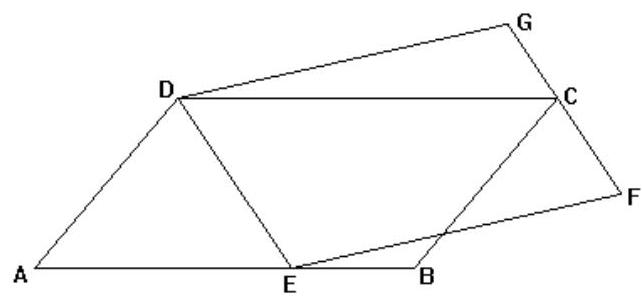
\includegraphics[max width=\textwidth, center]{2024_11_21_553e22f22be5e1eb25b0g-1}


\end{document}